\clearpage
\myparagraphold{Первый пример с \olly: a=1,2 и b=3,4}
\myindex{\olly}

Загружаем пример в \olly:

\begin{figure}[H]
\centering
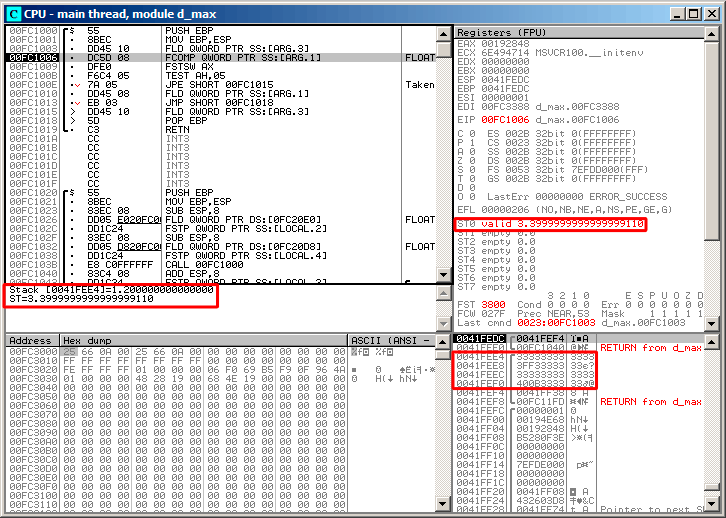
\includegraphics[scale=\FigScale]{patterns/12_FPU/3_comparison/x86/MSVC/olly1_1.png}
\caption{\olly: первая \FLD исполнилась}
\label{fig:FPU_comparison_case1_olly1}
\end{figure}

Текущие параметры функции: $a=1,2$ и $b=3,4$ 
(их видно в стеке: 2 пары 32-битных значений).
$b$ (3,4) уже загружено в \ST{0}.
Сейчас будет исполняться \FCOMP. 
\olly показывает второй аргумент для \FCOMP, который сейчас находится в стеке.

\clearpage
\FCOMP отработал:

\begin{figure}[H]
\centering
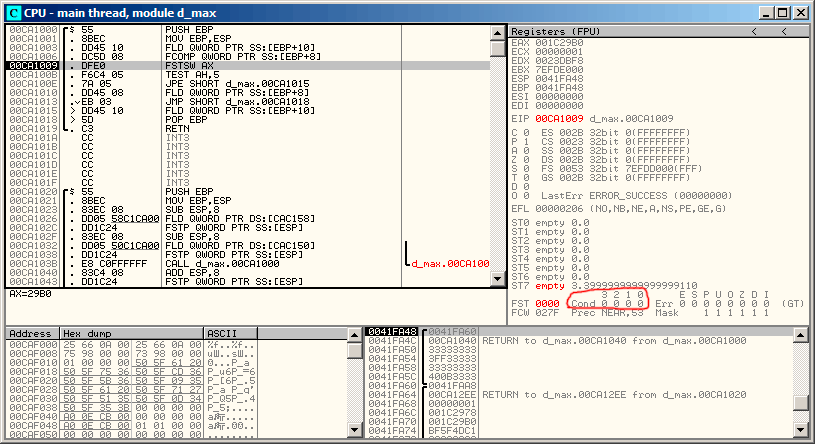
\includegraphics[scale=\FigScale]{patterns/12_FPU/3_comparison/x86/MSVC/olly1_2.png}
\caption{\olly: \FCOMP исполнилась}
\label{fig:FPU_comparison_case1_olly2}
\end{figure}

Мы видим состояния condition-флагов \ac{FPU}: 
все нули.
Вытолкнутое значение отображается как \ST{7}. Почему это так, объяснялось ранее%
: 
\myref{FPU_is_rather_circular_buffer}.

\clearpage
\FNSTSW сработал:
\begin{figure}[H]
\centering
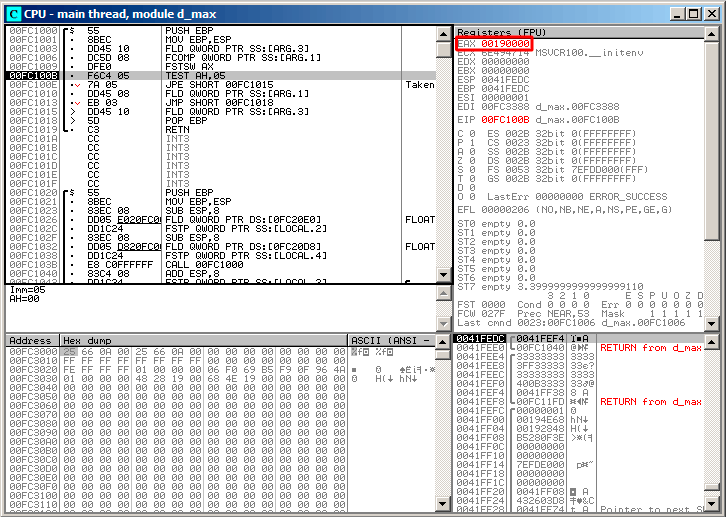
\includegraphics[scale=\FigScale]{patterns/12_FPU/3_comparison/x86/MSVC/olly1_3.png}
\caption{\olly: \FNSTSW исполнилась}
\label{fig:FPU_comparison_case1_olly3}
\end{figure}

Видно, что регистр \GTT{AX} содержит нули. Действительно, ведь все condition-флаги тоже содержали нули.

(\olly дизассемблирует команду \FNSTSW как \INS{FSTSW}~---%
 это синоним).

\clearpage
\TEST сработал:

\begin{figure}[H]
\centering
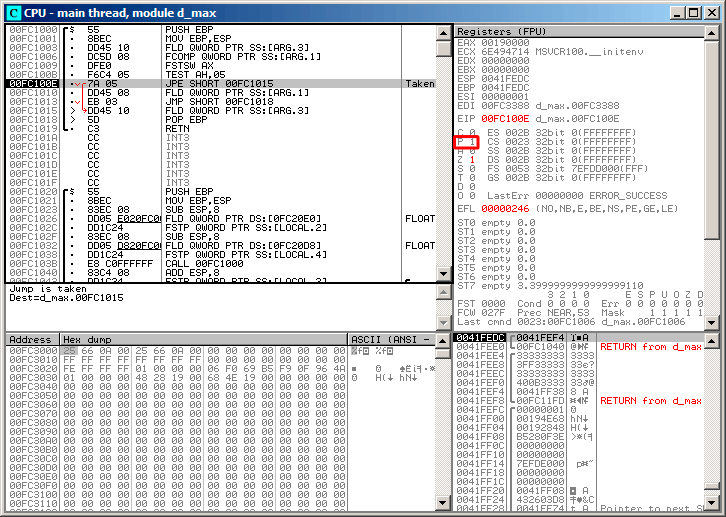
\includegraphics[scale=\FigScale]{patterns/12_FPU/3_comparison/x86/MSVC/olly1_4.png}
\caption{\olly: \TEST исполнилась}
\label{fig:FPU_comparison_case1_olly4}
\end{figure}

Флаг \GTT{PF} равен единице.
Всё верно: количество выставленных бит в 0~--- это 0, а 0~--- это четное число.

\olly дизассемблирует \INS{JP} как \ac{JPE}~--- это синонимы.
И она сейчас сработает.

\clearpage
\ac{JPE} сработала, \FLD загрузила в \ST{0} значение $b$ (3,4)%
:

\begin{figure}[H]
\centering
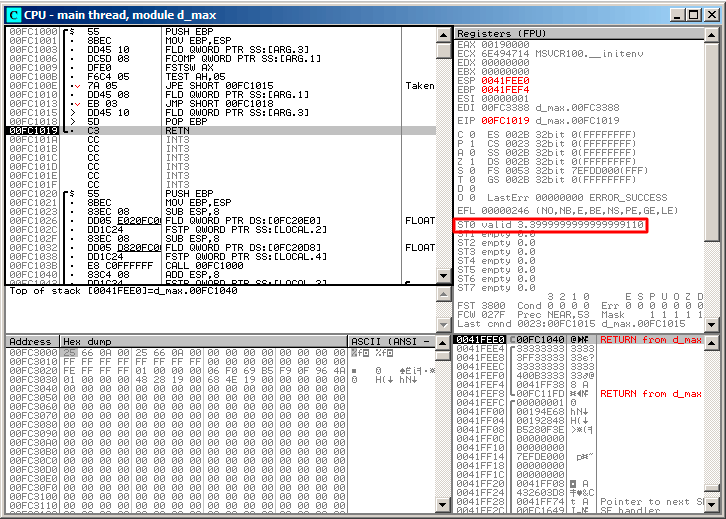
\includegraphics[scale=\FigScale]{patterns/12_FPU/3_comparison/x86/MSVC/olly1_5.png}
\caption{\olly: вторая \FLD исполнилась}
\label{fig:FPU_comparison_case1_olly5}
\end{figure}

Функция заканчивает свою работу.

\clearpage
\myparagraphold{Второй пример с \olly: a=5,6 и b=-1}

Загружаем пример в \olly:

\begin{figure}[H]
\centering
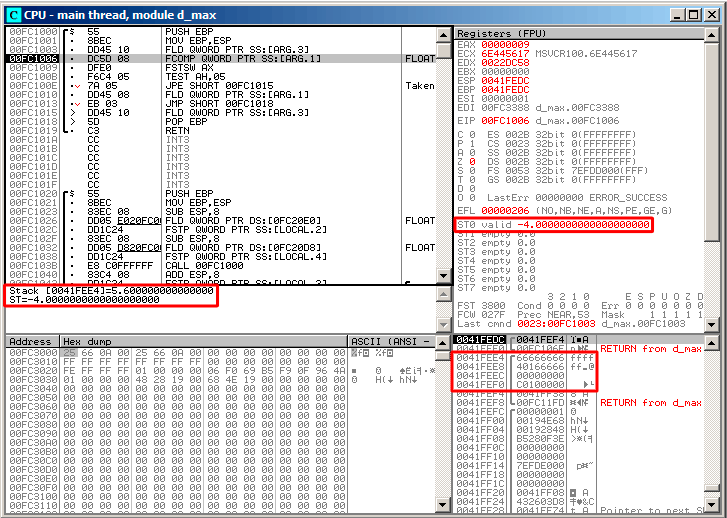
\includegraphics[scale=\FigScale]{patterns/12_FPU/3_comparison/x86/MSVC/olly2_1.png}
\caption{\olly: первая \FLD исполнилась}
\label{fig:FPU_comparison_case2_olly1}
\end{figure}

Текущие параметры функции: $a=5,6$ и $b=-4$.
$b$ (-4) уже загружено в \ST{0}.
Сейчас будет исполняться \FCOMP. 
\olly показывает второй аргумент \FCOMP, который сейчас находится в стеке.


\clearpage
\FCOMP отработал:

\begin{figure}[H]
\centering
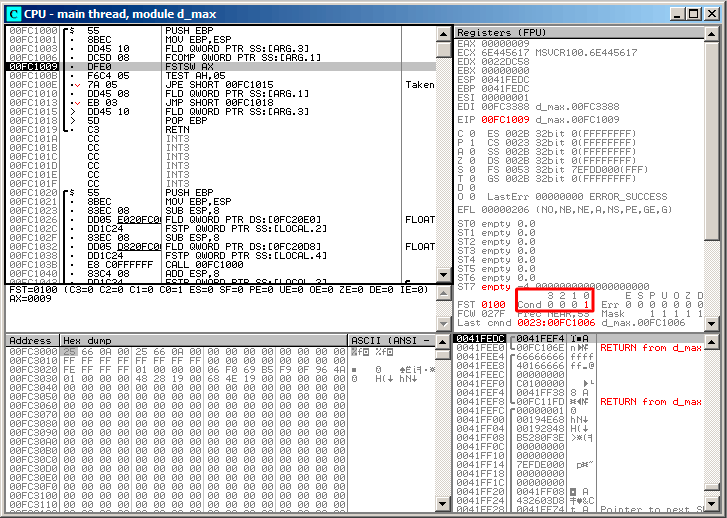
\includegraphics[scale=\FigScale]{patterns/12_FPU/3_comparison/x86/MSVC/olly2_2.png}
\caption{\olly: \FCOMP исполнилась}
\label{fig:FPU_comparison_case2_olly2}
\end{figure}

Мы видим значения condition-флагов \ac{FPU}: все нули, кроме \Czero.


\clearpage
\FNSTSW сработал:

\begin{figure}[H]
\centering
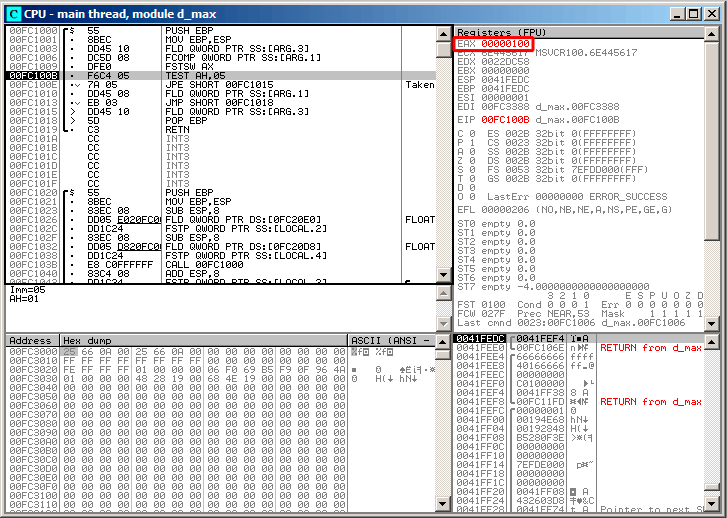
\includegraphics[scale=\FigScale]{patterns/12_FPU/3_comparison/x86/MSVC/olly2_3.png}
\caption{\olly: \FNSTSW исполнилась}
\label{fig:FPU_comparison_case2_olly3}
\end{figure}

Видно, что регистр \GTT{AX} содержит \GTT{0x100}: флаг \Czero стал на место 16-го бита.


\clearpage
\TEST сработал:

\begin{figure}[H]
\centering
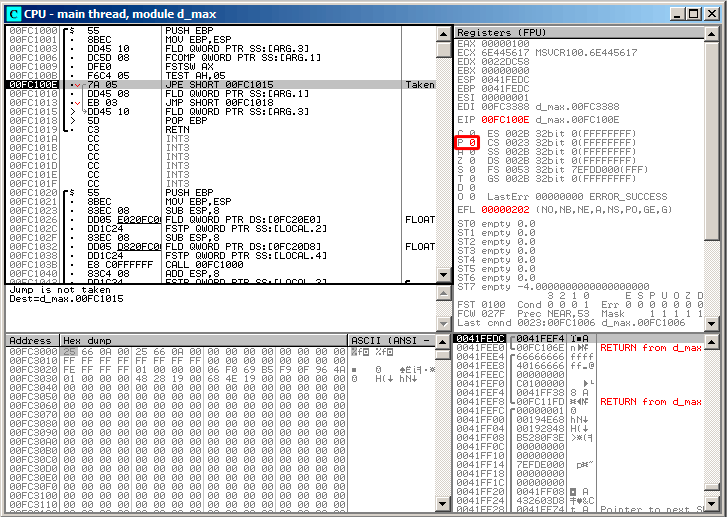
\includegraphics[scale=\FigScale]{patterns/12_FPU/3_comparison/x86/MSVC/olly2_4.png}
\caption{\olly: \TEST исполнилась}
\label{fig:FPU_comparison_case2_olly4}
\end{figure}

Флаг \GTT{PF} равен нулю.
Всё верно: 
количество единичных бит в \GTT{0x100}~--- 1, а 1~--- нечетное число.

\ac{JPE} сейчас не сработает.

\clearpage
\ac{JPE} не сработала,  \FLD 
загрузила в \ST{0} значение $a$ (5,6)%
:

\begin{figure}[H]
\centering
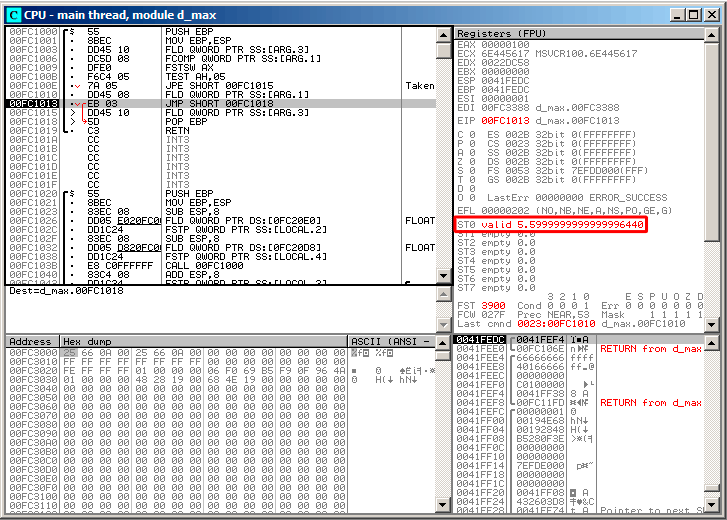
\includegraphics[scale=\FigScale]{patterns/12_FPU/3_comparison/x86/MSVC/olly2_5.png}
\caption{\olly: вторая \FLD исполнилась}
\label{fig:FPU_comparison_case2_olly5}
\end{figure}

Функция заканчивает свою работу.
